% begin module differentials-intro
\begin{frame}
\frametitle{(3.9)  Linear Approximations and Differentials}
\begin{itemize}
\item  Main idea: A curve is very close to its tangent line at the point of tangency.
\item  We can use the tangent line at $(a,f(a))$ as an approximation to the curve $y = f(x)$.
\item  This approximation works well as long as $x$ is near $a$.
\end{itemize}
\begin{center}
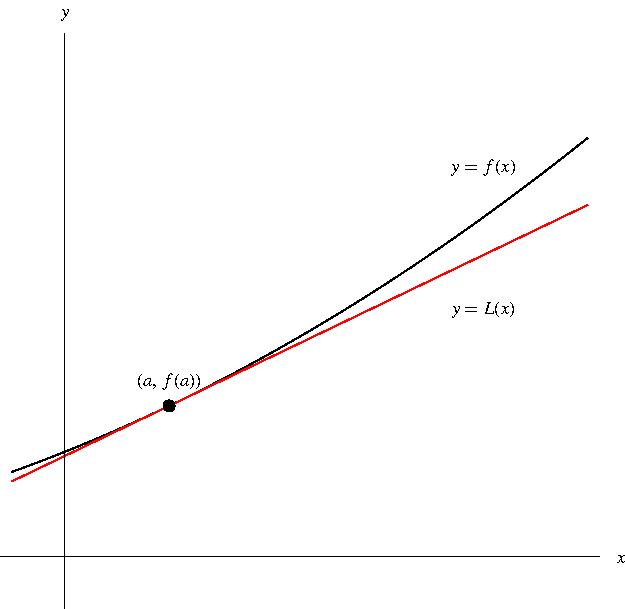
\includegraphics[height=4cm]{differentials/pictures/03-09-linapprox.pdf}%
\end{center}
\end{frame}
% end module differentials-intro
